\documentclass[conference]{IEEEtran}
\IEEEoverridecommandlockouts
% The preceding line is only needed to identify funding in the first footnote. If that is unneeded, please comment it out.
\usepackage{cite}
\usepackage{hyperref}
\usepackage{graphicx}
\usepackage[brazilian]{babel}
\usepackage[utf8]{inputenc}
\def\BibTeX{{\rm B\kern-.05em{\sc i\kern-.025em b}\kern-.08em
    T\kern-.1667em\lower.7ex\hbox{E}\kern-.125emX}}
\begin{document}

\title{Análise comparativa entre profissionais de tecnologia do setor público e privado dado o impacto da COVID-19 \\
}
\author{
	\IEEEauthorblockN{Marcelo Anselmo}
	\IEEEauthorblockA{
		\textit{Departamento de Ciência da}\\ 
		\textit{Computação}\\ 
		\textit{Universidade de Brasília}\\ 
		Brasília, Brasil \\
	marcelofilho@mpf.mp.br}
	\and
	\IEEEauthorblockN{Arivaldo Gonçalves}
	\IEEEauthorblockA{
		\textit{Departamento de Ciência da}\\ 
		\textit{Computação}\\ 
		\textit{Universidade de Brasília}\\ 
		Brasília, Brasil \\
	arivaldofreitas@correios.com.br}
	\and
	\IEEEauthorblockN{Luciana Maria}
	\IEEEauthorblockA{
		\textit{Departamento de Ciência da}\\ 
		\textit{Computação}\\ 
		\textit{Universidade de Brasília}\\ 
		Brasília, Brasil \\
	luciana@mpdft.mp.br}
	\and
	\IEEEauthorblockN{Marcelo Ladeira}
	\IEEEauthorblockA{
		\textit{Departamento de Ciência da}\\ 
		\textit{Computação}\\ 
		\textit{Universidade de Brasília}\\ 
		Brasília, Brasil \\
	mladeira@unb.br}
}

\maketitle
 
\begin{abstract}
	Este estudo aborda a diferença salarial entre homens e mulheres na área de TI durante a pandemia. Ele também explora possíveis cenários para analisar a disparidade salarial e de desligamento entre gêneros na área de tecnologia, antes e após a pandemia. Utilizou-se dados no nível do indivíduo, de 2018 a 2021, obtidos da Relação Anual de Informações Sociais (Rais), que proporciona dados oficiais sobre o mercado de trabalho no Brasil. No geral, constatou-se que a remuneração média das mulheres é menor que a dos homens em todas as regiões do Brasil, tanto em 2019 quanto em 2020. Além disso, a quantidade de desligamento de homens é maior que a de mulheres em todas as regiões do Brasil, tanto em 2019 quanto em 2020.
\end{abstract}

\begin{IEEEkeywords}
	Tecnologia da informação. Profissionais de TI. Diferença salarial. Gênero. Pandemia. COVID-19.
\end{IEEEkeywords}

\section{Introdução}

Com o avanço exponencial das tecnologias modernas, que estão modificando rapidamente as indústrias e sociedades globalmente, espera-se que a maneira como as pessoas trabalham, vivem e interagem com as outras seja transformada em uma velocidade e escala sem precedentes históricos \cite{hand1981artificial}. As inovações tecnológicas estão realmente mudando velozmente a fronteira entre as tarefas executadas por pessoas e por máquinas , transformando o mundo do trabalho \cite{aksoy2021robots}. O que não se sabe é se essas transformações estão também remodelando aspectos socioeconômicos, como as diferenças salariais entre gêneros.

A proteção do trabalho da mulher é assegurada pela Consolidação das Leis Trabalhistas (CLT), de 1943. Além disso, existe a Lei 9.029, de 1999, que instituiu regras sobre o acesso da mulher ao mercado de trabalho. Esse dispositivo proíbe, por exemplo, o anúncio de vagas de emprego com referência ao sexo ou que o sexo da pessoa seja uma variável determinante para fins de remuneração e oportunidades de ascensão profissional. No entanto, a diferença de remuneração entre homens e mulheres, que vinha em tendência de queda até 2020, voltou a subir no país e atingiu 22\% no fim de 2022, segundo dados do Instituto Brasileiro de Geografia e Estatística (IBGE). Isso significa que uma brasileira recebe, em média, 78\% do que ganha um homem.

Do ponto de vista de \cite{ahmed2015human}, é evidente a discriminação no mercado de trabalho contra as mulheres que, quando possuem as mesmas características dos homens em relação ao capital humano e desempenham a mesma atividade, recebem remuneração diferente em razão de seu sexo. Além disso, o relatório de 2015 da Organização das Nações Unidas (ONU) mostra que a assimetria salarial de sexo em favor dos homens ocorre em todas as indústrias e ocupações na maioria dos 177 países observados \cite{report2015onu}.

Dentro desse contexto, propõe-se verificar, neste estudo, se essa desigualdade salarial é também percebida entre os profissionais da área de Tecnologia da Informação (TI) em todo o território brasileiro, além de identificar se há uma diferença na quantidade de demissões. Para isso, utilizou-se dados da Relação Anual de Informações Sociais (RAIS) de 2015 a 2021, que fornece dados oficiais sobre o mercado de trabalho no Brasil. 

Sem pretender desmerecer as variadas identidades de gênero, neste artigo, os dados de sexo serão usados indiscriminadamente, pois os dados empíricos da pesquisa são binários. 

O trabalho está organizado da seguinte forma: Seção II, que trata do referencial teórico; Seção III, que apresenta os trabalhos correlatos; na Seção IV, a metodologia utilizada e os passos para exibir os dados estatísticos; na Seção V são apresentados os resultados obtidos e, pro fim, na Seção VI está a conclusão.
\section{Referêncial Teórico}
\subsection{Relação Anual de Informações Sociais (RAIS)}

A gestão pública brasileira, no setor trabalhista, possui um importante instrumento de coleta de dados denominado RAIS \cite{Sobre_a_RAIS}. Ele proporciona dados oficiais sobre o mercado de trabalho brasileiro. Tem por objetivo o suprimento às necessidades de controle da atividade trabalhista no País, o provimento de dados para a elaboração de estatísticas do trabalho e a disponibilização de informações do mercado de trabalho às entidades governamentais.

\subsection{Classificação Nacional de Atividades Econômicas (CNAE) e Classificação Brasileira de Ocupações (CBO)}

A CNAE \cite{Sobre_a_CNAE} é a classificação oficialmente adotada pelo Sistema Estatístico Nacional e pelos órgãos federais gestores de registros administrativos. Tem como aplicações: sistema estatístico, cadastro central de empresas, pesquisas econômicas estruturais, entre outros. Já a CBO \cite{Sobre_a_CBO} é um documento que retrata a realidade das profissões do mercado de trabalho brasileiro. 

Conforme os grupos CNAE que estão relacionados a atividades de TI, foram encontrados os códigos: Atividades dos serviços de tecnologia da informação (620) e Tratamento de dados, hospedagem na Internet e outras atividades relacionadas (631). Com esses grupos em mãos, foi possível encontrar suas respectivas ocupações, conforme podemos ver abaixo na tabela \ref{ocupacoes}.

\begin{table}[htbp]
	\caption{Ocupações analisadas}
	\begin{center}
		\begin{tabular}{|c|c|}
			\hline
			\textbf{Código} & \textbf{Descrição}                                  \\ 
			\hline
			212205           & Engenheiro de Aplicativos em Computacao               \\
			212210           & Engenheiro de Equipamentos em Computacao              \\
			212215           & Engenheiros de Sistemas Operacionais em Computacao    \\
			\hline 										
			212305           & Administrador de Banco de Dados                       \\
			212310           & Administrador de Redes                                \\
			212315           & Administrador de Sistemas Operacionais                \\
			212320           & Administrador em Segurança da Informação           \\
			\hline 									
			212405           & Analista de Desenvolvimento de Sistemas               \\
			212410           & Analista de Redes e de Comunicacao de Dados           \\
			212415           & Analista de Sistemas de Automacao                     \\
			212420           & Analista de Suporte Computacional                     \\
			\hline 									
			317105           & Programador de Internet                               \\
			317110           & Programador de Sistemas de Informacao                 \\
			317115           & Programador de Maquinas - Ferramenta com Comando Num. \\
			317120           & Programador de Multimidia                             \\
			\hline 									
			317205           & Operador de Computador (Inclusive Microcomputador)    \\
			317210           & Tecnico de Apoio ao Usuario de Informatica (Helpdesk) \\
			\hline
		\end{tabular}
		\label{ocupacoes}
	\end{center}
\end{table}

\subsection{Salário}

O salário é a remuneração que o empregado recebe pelo trabalho que realiza em uma instituição, pública ou privada. Segundo \cite{kryscynski2021firm}, os trabalhadores e suas empresas se envolvem em recorrentes relações de troca; de um lado, o trabalhador entrega valor, de outro, uma das recompensas que a empresa oferece em troca é o salário.
Considerando a relevância dessa temática na sociedade, é importante analisar a 
 desigualdade salarial, sobreduto entre grupos com alta dispersão salarial, seja em de nível educacional, raça, gênero etc. Este trabalho apresentará um diagnóstico com ênfase no sexo dentro dos vários cargos da área de TI, conforme apresentado na tabela \ref{ocupacoes}. 
\section{Trabalhos Relacionados}

No artigo \cite{ceballos2021airline}, os autores analisam o hiato de gênero na indústria de transformação brasileira para diferentes quantis da distribuição de salários de homens e mulheres. Em todos os estratos de produtividade, verificou-se um diferencial de rendimentos desfavorável às mulheres.

Os resultados também sugerem que as mulheres com alto nível de
qualificação seriam atraídas para os setores mais produtivos, entretanto, como foi observado, esses mesmos setores apresentam uma baixa representatividade feminina nos cargos de chefia, aqueles que comumente oferecem maiores rendimentos.

\section{Metodologia}

Todo o estudo proposto será realizado seguindo a metodologia Cross Industry Standard Process for Data Mining - CRISP-DM \cite{chapman2000crisp}, que é um processo padrão para mineração de dados.  Cabe destacar que não é proprietário e pretende ser independente do setor e das aplicações em que é utilizado.

O CRISP-DM envolve um ciclo faseado para um projeto ou pesquisa de mineração de dados. As atividades que compreendem este artigo serão realizadas conforme as seguintes etapas do CRISP-DM a seguir:

\begin{enumerate}
	\item Compreensão do negócio: Análise detalhada do tema "diferença de gênero" e a área de TI.
	\item Compreensão dos dados: os dados do RAIS serão coletados e examinados para identificar problemas de qualidade e verificar se eles são adequados para atender aos objetivos da pesquisa. Além disso, serão identificadas as variáveis que serão utilizadas na análise.
	\item Preparação dos dados: os dados da RAIS serão preparados para análise, o que pode incluir a limpeza de dados, a transformação de variáveis e a seleção de subconjuntos de dados relevantes. 
	\item Modelagem: serão aplicados modelos estatísticos para identificar padrões nos dados da RAIS, bem como relações entre variáveis.
	\item Avaliação: os resultados da modelagem serão avaliados para verificar se eles atendem aos objetivos da pesquisa, isto é, se eles fornecem informações úteis.
	\item Implantação: nesta etapa final, os resultados serão apresentados e as hipóteses confirmadas ou refutadas. 
\end{enumerate}
	      	      	      
\subsection{Compreensão dos dados}
	      	      	    
A análise foi feita com foco em quatro grupos, conforme a lista abaixo:

\begin{itemize}
	\item Nível educacional 	      	      	      	      	      
	\item Setor privado e público	      	      	      	      	     
	\item Quantidade de demissões    	      	      	      	     
	\item Diferença entre cargos de TI, conforme a tabela CBO \ref{ocupacoes}    	      	      	     
\end{itemize}
	      	      	    
Cada grupo foi analisado com base em duas variáveis:

\begin{itemize}
	\item Quantidade de pessoas do sexo masculino e feminino	      	      	      	      	      
	\item Salário médio ao longo de um ano	    
\end{itemize}
	      	      	      
A seguir, resumimos os dados analisados em uma tabela \ref{vars}:     

\begin{table}[htbp]
	\caption{Dados analisados}
	\begin{center}
		\begin{tabular}{|c|c|c|}
			\hline
			\textbf{Variável}           & \textbf{Definição}        & \textbf{Exemplo}       \\ 
			\hline 
			\textbf{Ano}                 & Período dos dados          & 2018, 2019             \\
			\hline
			\textbf{Sexo}                & Masculino ou Feminino       & 1 ou 2                 \\
			\hline
			\textbf{Salário}            & Com base no ano             & 5000                   \\
			\hline 
			\textbf{Tipo de vínculo}    & Setor Privado ou Público   & CLT, Estatutário      \\
			\hline 
			\textbf{Motivo Desligamento} & Demissão, falecimento, etc & Com acordo, sem acordo \\
			\hline
			\textbf{Ocupação}          & Descrição do cargo        & Analista de suporte    \\
			\hline 
		\end{tabular}
		\label{vars}
	\end{center} 
\end{table}      	      

\subsection{Preparação dos dados}

Foi feito um processo de Extração, Transformação e Carga (ETL) para preparar os dados para análise. O processo foi feito com a linguagem Python e a análise com a biblioteca Pandas. A fonte de dados da RAIS foi extraída a partir do site basedosdados.org \cite{basedosdados}, utilizando a API disponível através da plataforma BigQuery \cite{bigquery}. Os dados extraídos compreendem o período de 2015 a 2021, pois foram os dados disponibilizados para este estudo sem custos adicionais da plataforma BigQuery. 

\subsection{Modelagem}

A modelagem foi feita com base em gráficos de barras, de linhas, e de mapas. Os gráficos de barras e de linhas foram utilizados para mostrar a quantidade de pessoas do sexo masculino e feminino, bem como o salário médio ao longo de um ano. Os mapas foram utilizados para mostrar a quantidade de pessoas do sexo masculino e feminino por estado.
\section{Resultados Obtidos}

As análises foram feitas entre os anos de 2018 e 2019 (pré COVID), e 2020 e 2021 (pós COVID). Conforme o cenário mundial mudou de um ano para o outro, percebemos que as diferenças entre os gêneros também mudaram.

\subsection{Remuneração Geral de 2018 a 2021}

A tabela abaixo \ref{remunTotal} nos mostra que a remuneração média das mulheres é menor ...

\begin{table}[htbp]
	\caption{Remuneração de 2018 a 2021}
	\begin{center}
		\begin{tabular}{|c|c|c|c|c|}
			\hline
			\textbf{Região} & \textbf{Sexo} & \textbf{Méd.} & \textbf{Dif} & \textbf{Dif\%} \\ 
			\hline																			
																																																																							
			Centro-Oeste     & Feminino      & 6542.79        &              &                \\ 
			                 & Masculino     & 7186.17        & 643.38       & 9.83\%         \\ \hline
			Nordeste         & Feminino      & 3900.37        &              &                \\ 
			                 & Masculino     & 3902.51        & 2.14         & 0.05\%         \\ \hline
			Norte            & Feminino      & 3060.56        &              &                \\ 
			                 & Masculino     & 4062.80        & 1002.24      & 32.75\%        \\ \hline
			Sudeste          & Feminino      & 5293.50        &              &                \\ 
			                 & Masculino     & 6094.63        & 801.13       & 15.13\%        \\ \hline
			Sul              & Feminino      & 4123.61        &              &                \\ 
			                 & Masculino     & 4745.27        & 621.66       & 15.08\%        \\ 
			\hline
		\end{tabular}
		\label{remunTotal}
	\end{center}
\end{table}

\subsection{Remuneração de 2018 a 2021}

A tabela abaixo \ref{remunTotal} nos mostra que a remuneração média das mulheres é menor ...

\begin{table}[htbp]
	\caption{Remuneração de 2018 a 2021}
	\begin{center}
		\begin{tabular}{|c|c|c|c|c|c|}
			\hline
			\textbf{Ano} & \textbf{Região} & \textbf{Sexo} & \textbf{Méd.} & \textbf{Dif} & \textbf{Dif\%} \\ 
			\hline																			
																																																																							
			2018         & Centro-Oeste     & Feminino      & 6979.09        &              &                \\
			             &                  & Masculino     & 6801.06        & -178.03      & -2.55\%        \\
			             & Nordeste         & Feminino      & 4247.12        &              &                \\
			             &                  & Masculino     & 4044.22        & -202.9       & -4.78\%        \\
			             & Norte            & Feminino      & 2859.67        &              &                \\
			             &                  & Masculino     & 4024.01        & 1164.34      & 40.72\%        \\
			             & Sudeste          & Feminino      & 5256.70        &              &                \\
			             &                  & Masculino     & 5985.95        & 729.25       & 13.87\%        \\
			             & Sul              & Feminino      & 4767.86        &              &                \\
			             &                  & Masculino     & 4996.56        & 228.7        & 4.8\%          \\ \hline
			2019         & Centro-Oeste     & Feminino      & 10576.11       &              &                \\
			             &                  & Masculino     & 9612.65        & -963.46      & -9.11\%        \\
			             & Nordeste         & Feminino      & 2848.94        &              &                \\
			             &                  & Masculino     & 3677.29        & 828.35       & 29.08\%        \\
			             & Norte            & Feminino      & 3390.81        &              &                \\
			             &                  & Masculino     & 3260.72        & -130.09      & -3.84\%        \\
			             & Sudeste          & Feminino      & 5271.16        &              &                \\
			             &                  & Masculino     & 5377.40        & 106.24       & 2.02\%         \\
			             & Sul              & Feminino      & 3905.04        &              &                \\
			             &                  & Masculino     & 4250.18        & 345.14       & 8.84\%         \\\hline
			2020         & Centro-Oeste     & Feminino      & 4287.08        &              &                \\
			             &                  & Masculino     & 6337.51        & 2050.43      & 47.83\%        \\
			             & Nordeste         & Feminino      & 3161.25        &              &                \\
			             &                  & Masculino     & 3481.98        & 320.73       & 10.15\%        \\
			             & Norte            & Feminino      & 3741.41        &              &                \\
			             &                  & Masculino     & 3161.25        & -580.16      & -15.51\%       \\
			             & Sudeste          & Feminino      & 4386.02        &              &                \\
			             &                  & Masculino     & 5285.72        & 899.7        & 20.51\%        \\
			             & Sul              & Feminino      & 3275.24        &              &                \\
			             &                  & Masculino     & 3942.60        & 667.36       & 20.38\%        \\\hline
			2021         & Centro-Oeste     & Feminino      & 5426.14        &              &                \\
			             &                  & Masculino     & 6782.73        & 1356.59      & 25.0\%         \\
			             & Nordeste         & Feminino      & 4077.23        &              &                \\
			             &                  & Masculino     & 4003.20        & -74.03       & -1.82\%        \\
			             & Norte            & Feminino      & 4177.48        &              &                \\
			             &                  & Masculino     & 4571.86        & 394.38       & 9.44\%         \\
			             & Sudeste          & Feminino      & 5541.26        &              &                \\
			             &                  & Masculino     & 6552.65        & 1011.39      & 18.25\%        \\
			             & Sul              & Feminino      & 4097.54        &              &                \\
			             &                  & Masculino     & 4981.30        & 883.76       & 21.57\%        \\
			\hline
		\end{tabular}
		\label{remunTotal}
	\end{center}
\end{table}

A tabela abaixo \ref{desligTotal} nos mostra que o desligamentos médios das mulheres é menor ...

\begin{table}[htbp]
	\caption{Desligamentos de 2018 a 2021}
	\begin{center}
		\begin{tabular}{|c|c|c|c|c|c|}
			\hline
			\textbf{Ano} & \textbf{Região} & \textbf{Sexo} & \textbf{Méd.} & \textbf{Dif} & \textbf{Dif\%} \\ 
			\hline																			
			2018         & Centro-Oeste     & Feminino      & 7475           &              &                \\
			             &                  & Masculino     & 27762          & 20287.0      & 271.4\%        \\
			             & Nordeste         & Feminino      & 7886           &              &                \\
			             &                  & Masculino     & 35368          & 27482.0      & 348.49\%       \\
			             & Norte            & Feminino      & 27383          &              &                \\
			             &                  & Masculino     & 31209          & 3826.0       & 13.97\%        \\
			             & Sudeste          & Feminino      & 45345          &              &                \\
			             &                  & Masculino     & 207928         & 162583.0     & 358.55\%       \\
			             & Sul              & Feminino      & 12363          &              &                \\
			             &                  & Masculino     & 59456          & 47093.0      & 380.92\%       \\\hline
			2019         & Centro-Oeste     & Feminino      & 3135           &              &                \\
			             &                  & Masculino     & 16455          & 13320.0      & 424.88\%       \\
			             & Nordeste         & Feminino      & 1796           &              &                \\
			             &                  & Masculino     & 9765           & 7969.0       & 443.71\%       \\
			             & Norte            & Feminino      & 801            &              &                \\
			             &                  & Masculino     & 1722           & 921.0        & 114.98\%       \\
			             & Sudeste          & Feminino      & 14399          &              &                \\
			             &                  & Masculino     & 70987          & 56588.0      & 393.0\%        \\
			             & Sul              & Feminino      & 3470           &              &                \\
			             &                  & Masculino     & 26534          & 23064.0      & 664.67\%       \\\hline
			2020         & Centro-Oeste     & Feminino      & 3001           &              &                \\
			             &                  & Masculino     & 15757          & 12756.0      & 425.06\%       \\
			             & Nordeste         & Feminino      & 3939           &              &                \\
			             &                  & Masculino     & 17567          & 13628.0      & 345.98\%       \\
			             & Norte            & Feminino      & 4031           &              &                \\
			             &                  & Masculino     & 4085           & 54.0         & 1.34\%         \\
			             & Sudeste          & Feminino      & 24390          &              &                \\
			             &                  & Masculino     & 103504         & 79114.0      & 324.37\%       \\
			             & Sul              & Feminino      & 7720           &              &                \\
			             &                  & Masculino     & 30439          & 22719.0      & 294.29\%       \\\hline
			2021         & Centro-Oeste     & Feminino      & 8182           &              &                \\
			             &                  & Masculino     & 39322          & 31140.0      & 380.59\%       \\
			             & Nordeste         & Feminino      & 11678          &              &                \\
			             &                  & Masculino     & 45432          & 33754.0      & 289.04\%       \\
			             & Norte            & Feminino      & 2231           &              &                \\
			             &                  & Masculino     & 12326          & 10095.0      & 452.49\%       \\
			             & Sudeste          & Feminino      & 97366          &              &                \\
			             &                  & Masculino     & 343299         & 245933.0     & 252.59\%       \\
			             & Sul              & Feminino      & 25201          &              &                \\
			             &                  & Masculino     & 95873          & 70672.0      & 280.43\%       \\
			\hline
		\end{tabular}
		\label{desligTotal}
	\end{center}
\end{table}
\section{Conclusões}

As tecnologias estão cada vez mais presentes na vida das pessoas, acarretando mudanças significativas no contexto profissional. Em outras palavras, a tecnologia está mudando a forma como as pessoas trabalham e como as empresas operam. Além disso, a tecnologia está mudando a natureza do trabalho, criando novas tarefas e alterando as existentes.

Com este presente estudo, concluímos que a remuneração média ...

Além de verificar o hiato de rendimentos de gênero na média salarial, também
é possível verificar o comportamento desse fenômeno ao longo da distribuição de
rendimentos por meio de análise quantílica. Esse tipo de abordagem mostra-se interessante por viabilizar a análise dos determinantes desse hiato para diferentes quantis da distribuição de salários, permitindo visualizar a evolução das desigualdades de rendimentos para diferentes níveis de renda e analisar os efeitos de variáveis explicativas para cada um desses níveis

No Brasil, a participação feminina em ocupações STEM é ainda menor, sendo de x\%.
 

\bibliographystyle{IEEEtran}
\bibliography{bibliografia}{}

% insert page break
\newpage

\section{Anexos}

\begin{figure}[htbp]
	\centerline{
		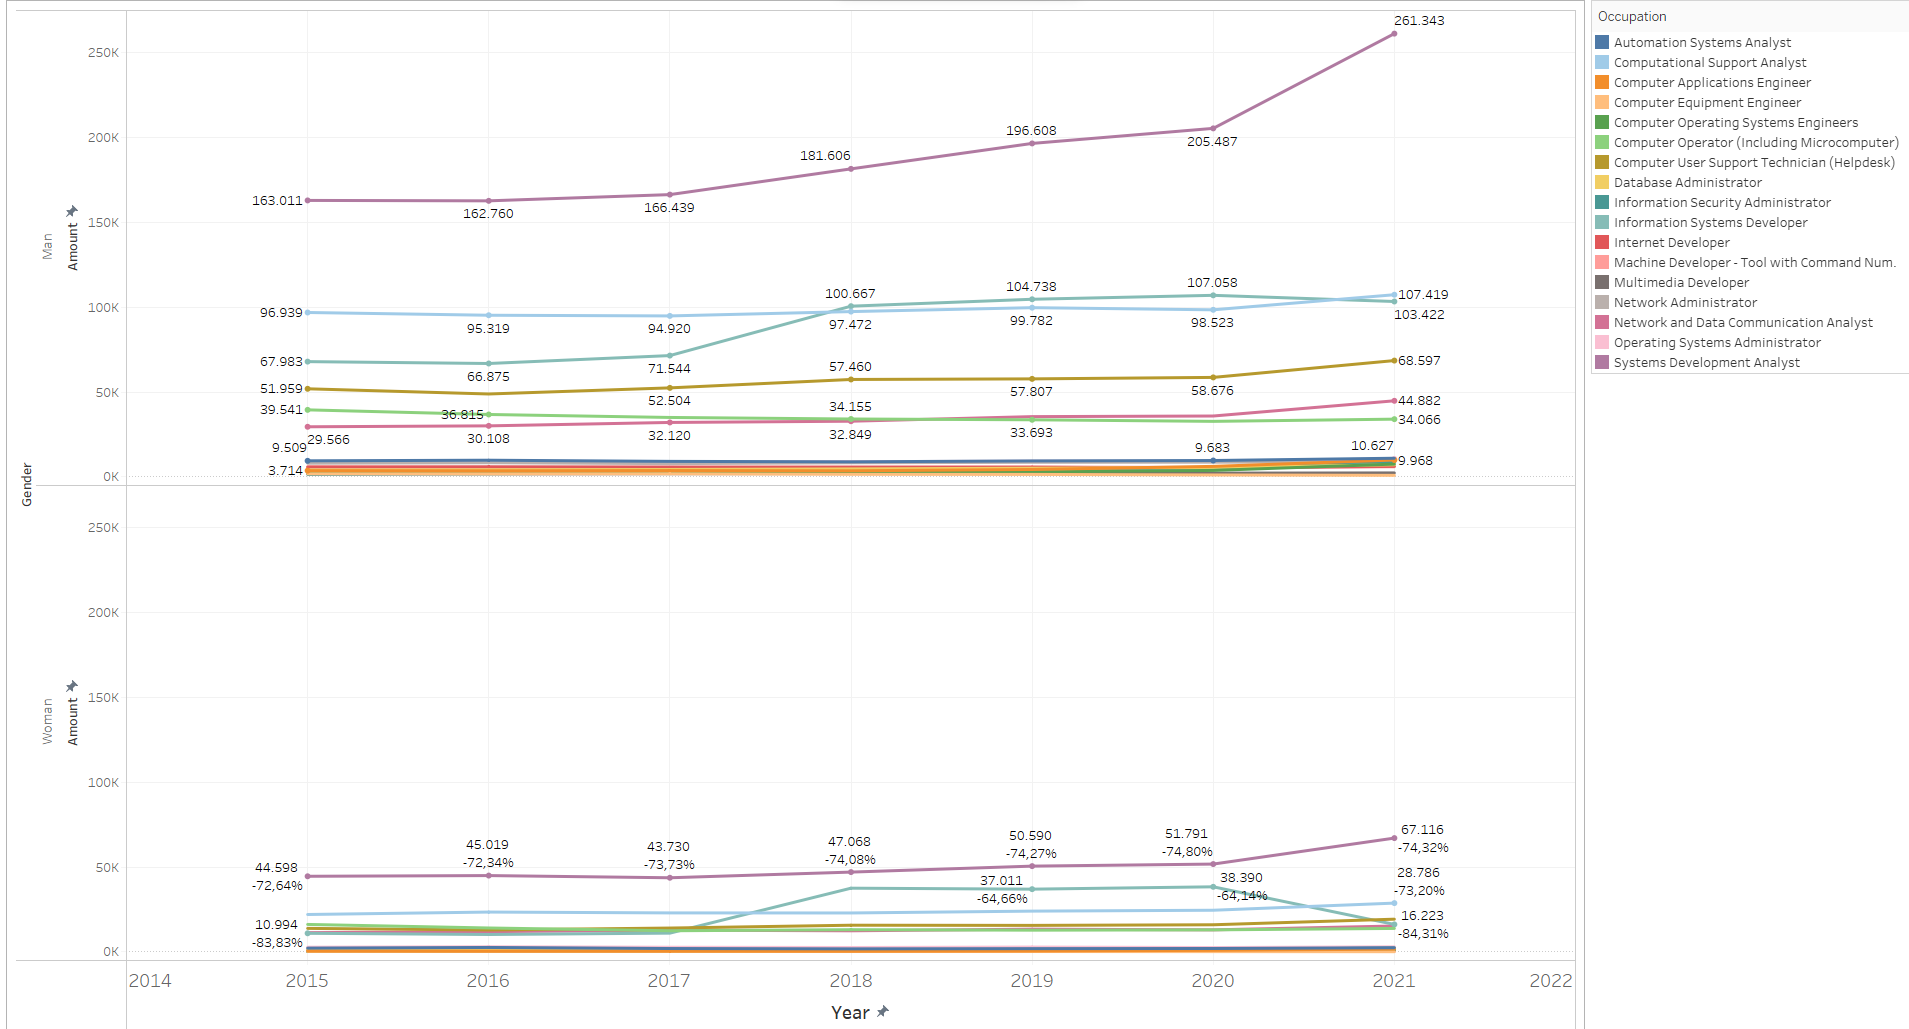
\includegraphics[width=250mm]{assets/5_qnt_cbo_full.PNG}
	}
	\caption{Locais onde a mulher ganha mais ou ganha menos que o homem}
	\label{fig_5_qnt_cbo_full}
\end{figure}

\begin{figure}[htbp]
	\centerline{
		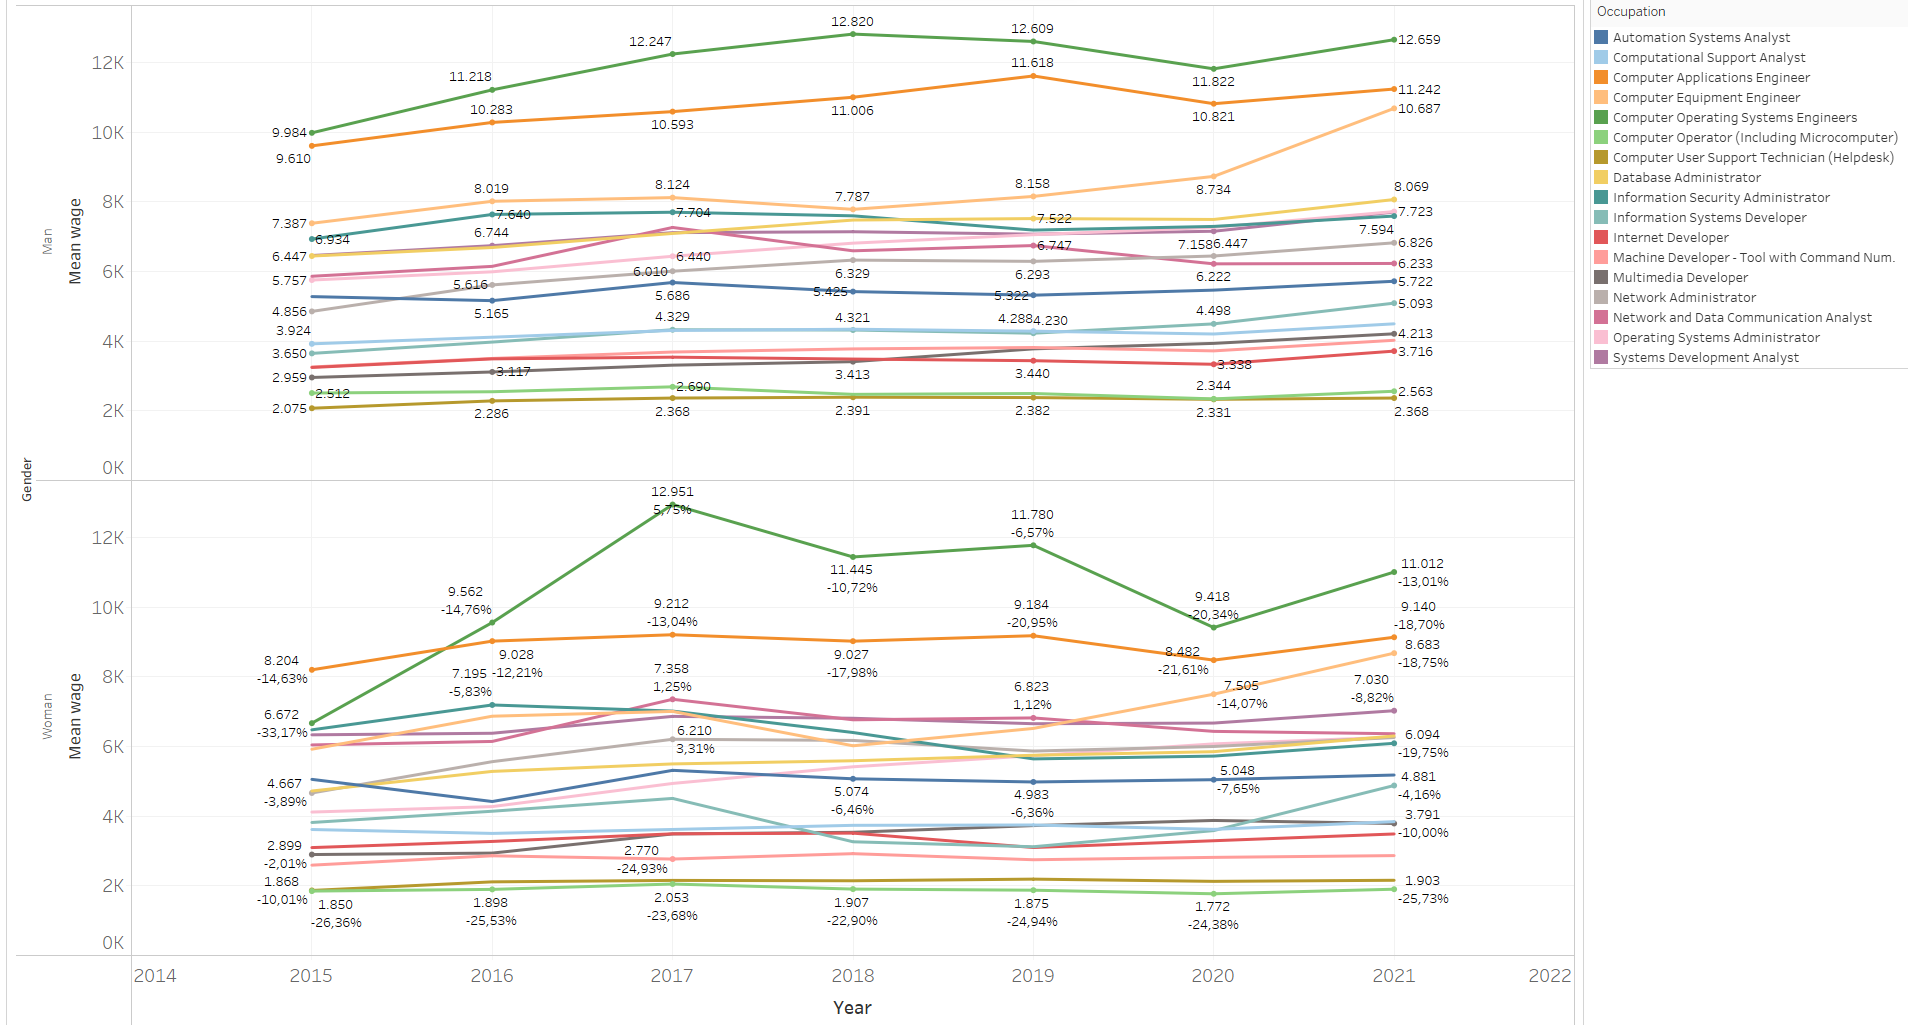
\includegraphics[width=85mm]{assets/5_sal_cbo_full.PNG}
	}
	\caption{Média salarial por cargo em todos os anos}
	\label{fig_5_sal_cbo_full}
\end{figure}



\begin{figure}[htbp]
	\centerline{
		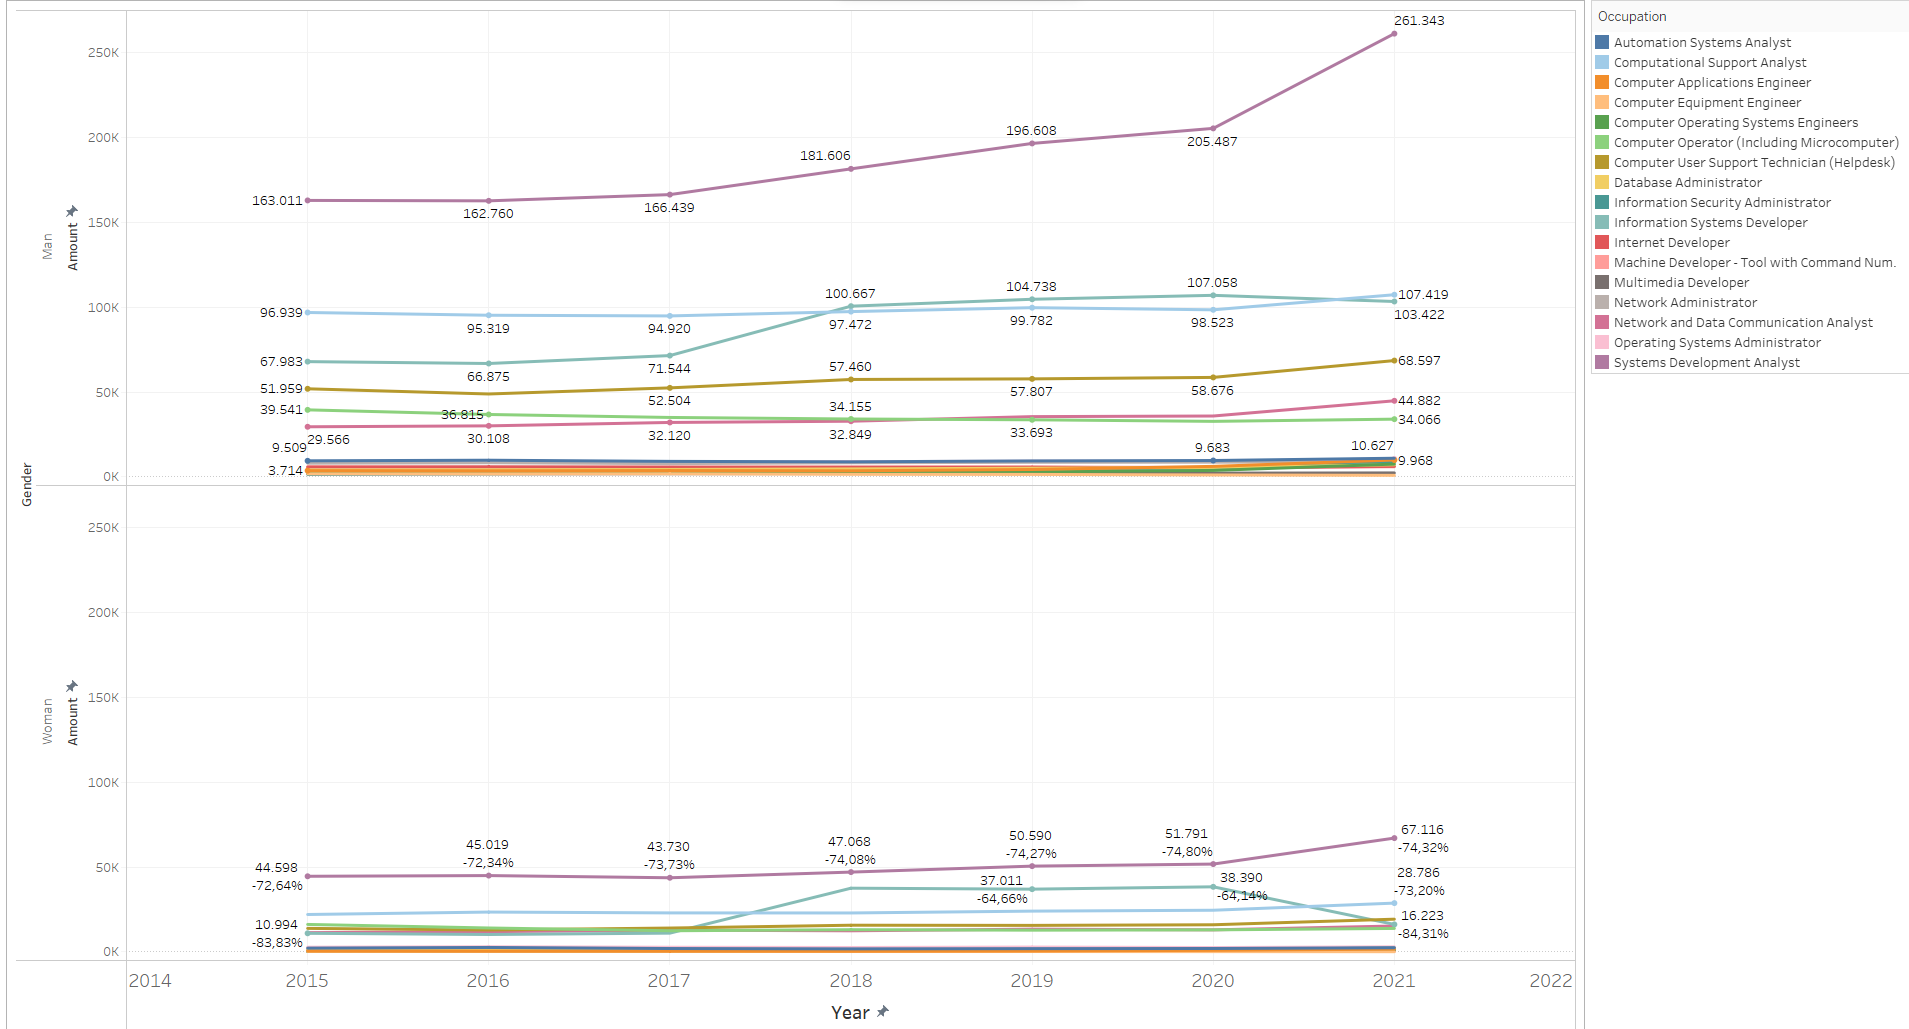
\includegraphics[width=250mm]{assets/5_qnt_cbo_full.PNG}
	}
	\caption{Quantidade por cargo em todos os anos}
	\label{fig_5_qnt_cbo_full}
\end{figure}

\begin{figure}[htbp]
	\centerline{
		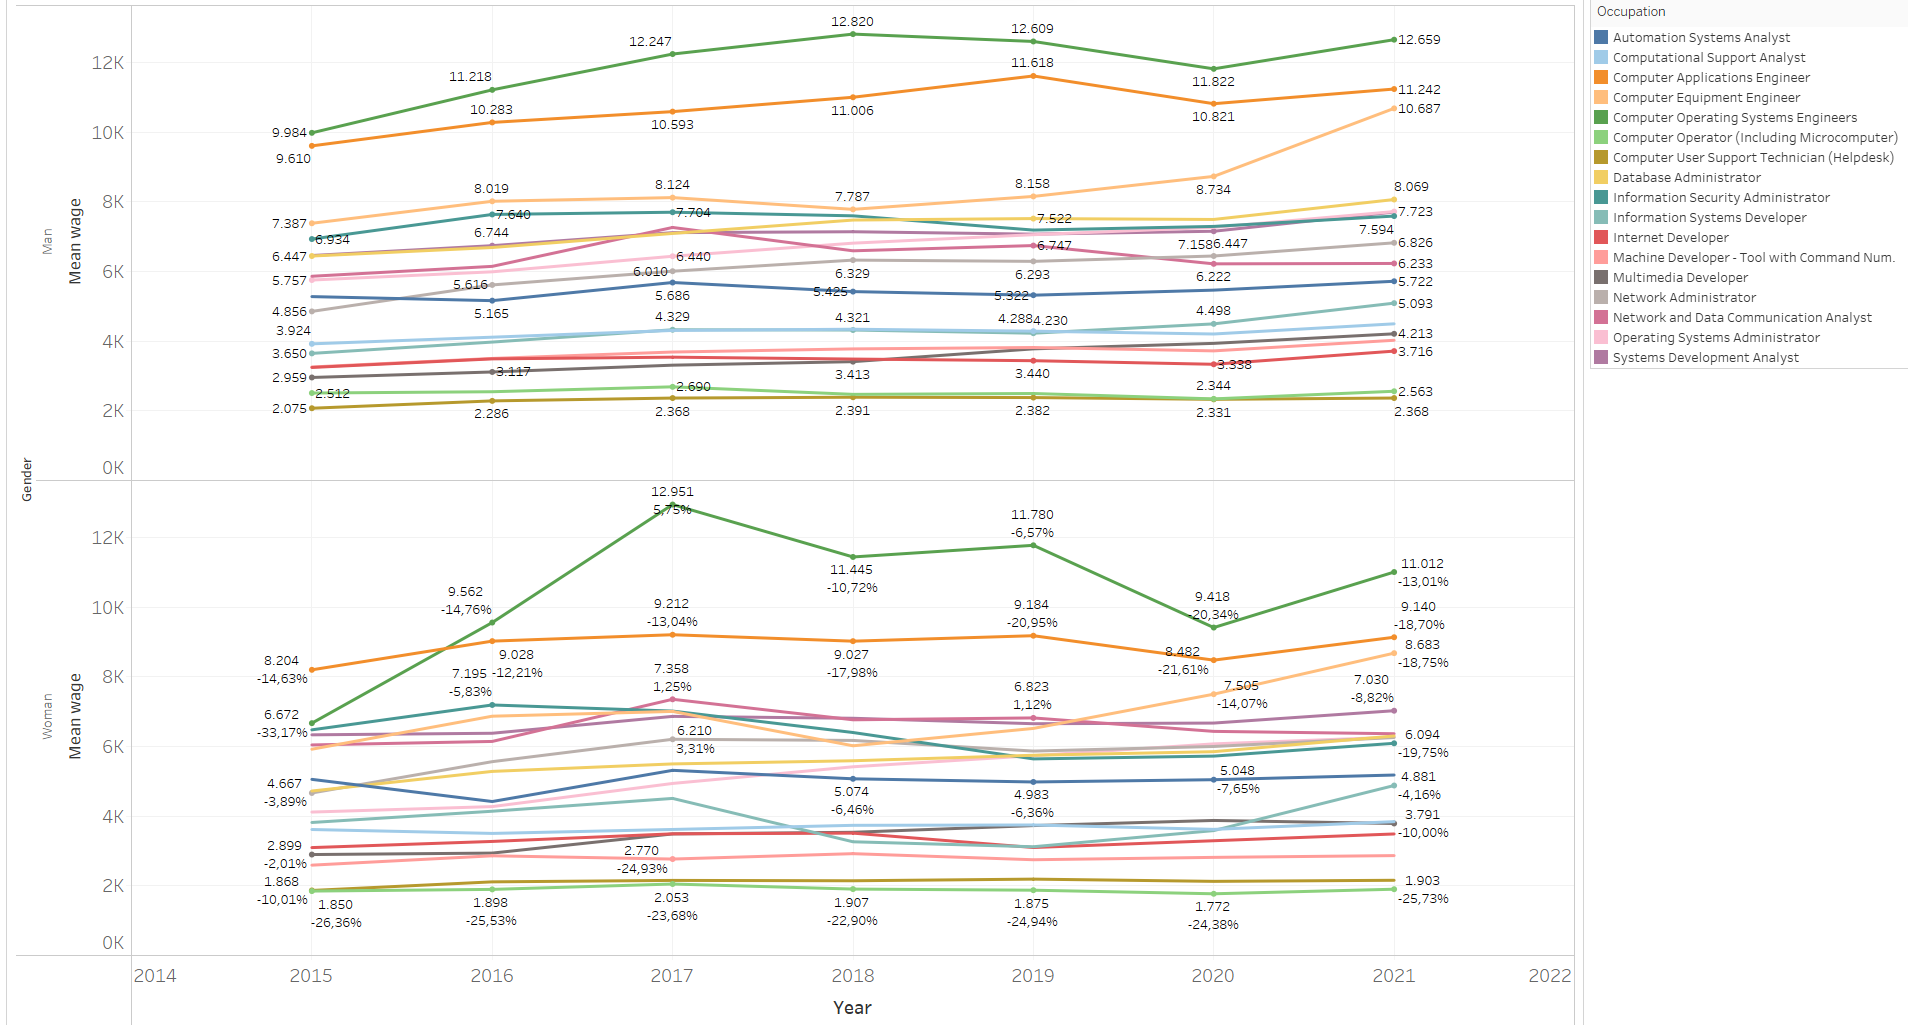
\includegraphics[width=85mm]{assets/5_sal_cbo_full.PNG}
	}
	\caption{Média salarial por cargo em todos os anos}
	\label{fig_5_sal_cbo_full}
\end{figure}



  

\end{document}
